\documentclass[a4paper,fleqn]{cas-dc}
\usepackage[english,russian]{babel}%используем русский и английский языки с переносами
\usepackage[numbers]{natbib}
\usepackage{lipsum}
\usepackage{floatrow}
\usepackage{graphicx}

\usepackage{booktabs}
\usepackage{multirow}

\graphicspath{{figs/}}

%%%Author definitions
\def\tsc#1{\csdef{#1}{\textsc{\lowercase{#1}}\xspace}}
\tsc{WGM}
\tsc{QE}
\tsc{EP}
\tsc{PMS}
\tsc{BEC}
\tsc{DE}
%%%

\begin{document}
\let\WriteBookmarks\relax
\def\floatpagepagefraction{1}
\def\textpagefraction{.001}
\title{Подбор оптимального метода для расчета электронной структуры и энергий 
ионизации $\beta$-дикетонов, их тио- и имино-аналогов}
\author%
[1]{Tikhonov}[type=editor,prefix=Sergey A.,]
\cormark[1]
%\cortext[cor1]{Corresponding author}
\address[1]{Russian Federation}

\author[2]{Samoilov}[prefix=Ilya S.]

\address[2]{Saint-Petersburg State University,
            Department of Photonics,
            St. Petersburg 199034,
            Russian Federation}
\begin{abstract}
\lipsum
\lipsum[3]
\end{abstract}

\begin{keywords}
Electronic structure \sep
Photoelectron spectroscopy \sep
UPS \sep
Density functional theory \sep
Outer-valence Green's function\\ (OVGF) method
\end{keywords}
\maketitle
\section{Introduction}
$\beta$-Дикетоны, их тио- и имино-аналоги~\cite{mcalduff1979photoelectron,evans1972study,joergensen1981electronic}
используются как прекурсоры при синтезе хелатных комплексов p-, d- и f-элементов~\cite{lutoshkin2021interaction},
которые обладают важными потребительскими свойствами и находят применение в качестве материалов для нужд фотоники~
\cite{zolotareva2013beta,sasabe2017unique}, сенсорики~\cite{lavis2014bright}, лазерной техники, биомедицины~
\cite{wang2021multi,lavis2008bright,klymchenko2017solvatochromic,grabowski2003structural,
kucherak2010switchable,klymchenko2014fluorescent}, полимерной инженерии~\cite{chen2014eva} и
солнечной энергетики~\cite{de1998novel}.
\par Понимание взаимосвязей <<строение-свойство>> даёт возможность осуществлять направленный синтез материалов с заранее заданными физическими свойствами. Выявление корреляций между электронной структурой валентных уровней и
 физическими характеристиками материала, с использованием современных методов квантовохимического моделирования, позволяет улучшить понимание взаимосвязей <<строение-свойство>>. Поэтому подбор оптимального метода расчёта электронной
структуры $\beta$-дикетонов и их производных является актуальной задачей.
\par Наиболее популярным расчётным методом является метод теории функционала плотности (ТФП), однако, ввиду допущений лежащих в основе метода, интерпретация расчётных данных и сопоставление их с экспериментальными результатами бывает
затруднено. Подбор оптимального функционала позволяет нивелировать недостатки расчётного метода и получить результаты сопоставимые с более точными, но и более ресурсозатратными методами, такими как метод функций Грина или связанных
кластеров.

\begin{figure}[ht]
\center{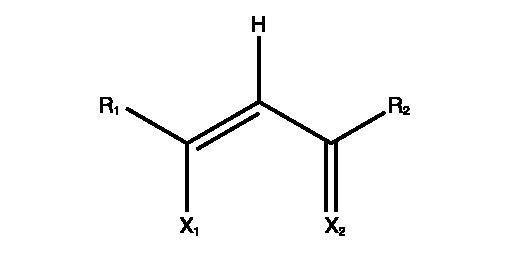
\includegraphics[width=1\linewidth]{Fig_1_Stroenie.pdf}}
\caption{Schematic representation of the studied complexes.}
\label{Ris_1_Structur_formula}
\end{figure}

\begin{table}[t]
\caption{Исследованные соединения}
\centering
\label{tab1}
\begin{tabular}{lllll}
\hline
Compound & X$_1$  & X$_2$  & R$_1$      & R$_2$      \\ \hline
I        & H      & O      & H          & H          \\
II       & H      & O      & CH$_3$     & CH$_3$     \\
III      & NH2    & O      & CH$_3$     & CH$_3$     \\
IV       & NHCH3  & O      & CH$_3$     & CH$_3$     \\
V        & SCH3   & O      & CH$_3$     & CH$_3$     \\
VI       & SH     & O      & CH$_3$     & CH$_3$     \\
VII      & OH     & S      & CH$_3$     & CH$_3$     \\
VIII     & OH     & O      & CF$_3$     & CH$_3$     \\
IX       & OH     & O      & CF$_3$     & CF$_3$     \\
X        & OH     & O      & C$_6$H$_5$ & C$_6$H$_5$ \\ \hline
\end{tabular}
\end{table}

\section{Experimental and theoretical methods}

\par Фотоэлектронные спектры соединений II-IV~\cite{Vovna_Grinc} были сняты на приборе ЭС-3201, c монохроматическим источником излучения He(I) (h$\nu$ = 21.2 eV), разрешение прибора составляло 50 мэВ, температура 20-40\,$^\circ$C.
Соединения V-VII сняты на спектрометре фирмы Perkin-Elmer PS-18, c монохроматическим источником излучения He(I), разрешение прибора составляло 25-35 meV.
Соединения VIII-IX сняты на спектрометре фирмы Perkin-Elmer PS-15 c монохроматическим источником излучения He(I).

\par Бенчмарк 19 функционалов осуществлялся в программном пакете GAMESS ~\cite{GAMESS} с использованием Dunning-type Correlation Consistent basis set cc-pVTZ. Для каждого соединения
выполнялась первичная пре-оптимизация геометрии в программном пакете Gaussian 16~\cite{g16} функционале B3LYP[ ] и базисном наборе def2svp[]. Затем выполнялась
основная оптимизация геометрии в B3LYP/def2tzvpp[]. Расчёты методом функций Грина, а именно OVGF[ ], P3[ ], P3+[ ] велись с использованием базисного набора cc-pvtz[ ].

\lipsum[3]


\begin{figure}[ht]
    \center{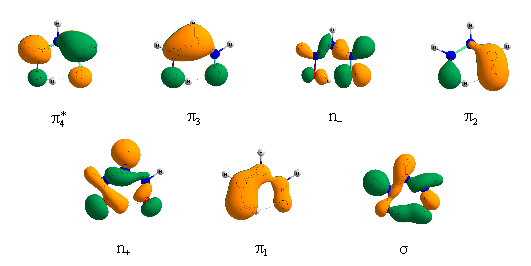
\includegraphics[width=1\linewidth]{Fig_4_orbitali_malanat.pdf}}
    \caption{Орбитали валентной области.}
    \label{Ris_4_orbitali_malanat}
    \end{figure}

\lipsum[7-8]

\begin{figure}[ht]
    \center{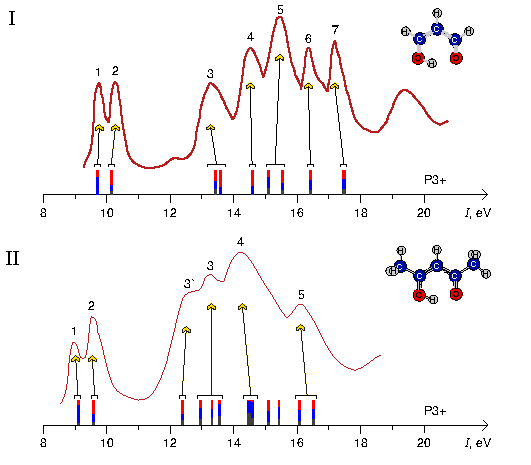
\includegraphics[width=1\linewidth]{Fig_5_UPS-1.pdf}}
    \caption{Рисунок спектров номер один.}
    \label{Ris_5_UPS_1}
    \end{figure}

\lipsum[9-12]

\begin{figure}[ht]
    \center{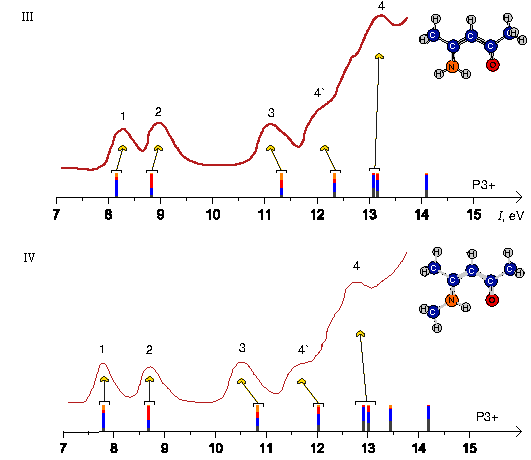
\includegraphics[width=1\linewidth]{Fig_6_UPS-2.pdf}}
    \caption{Рисунок спектров номер два.}
    \label{Ris_6_UPS_2}
    \end{figure}

\lipsum[10-11]

\begin{figure}[ht]
    \center{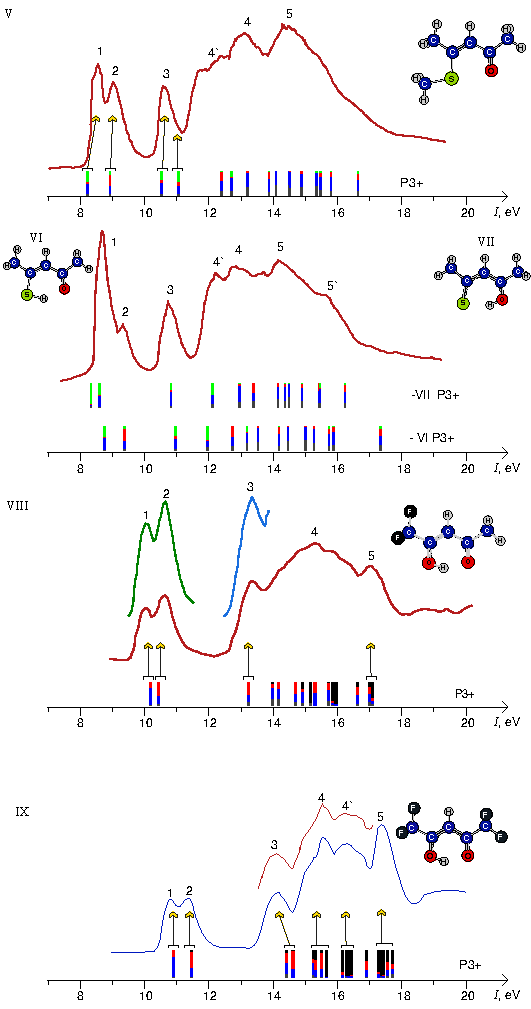
\includegraphics[width=1\linewidth]{Fig_7_UPS-3.pdf}}
    \caption{Рисунок спектров номер три.}
    \label{Ris_7_UPS_3}
    \end{figure}

\lipsum[12-13]

\begin{figure}[ht]
    \center{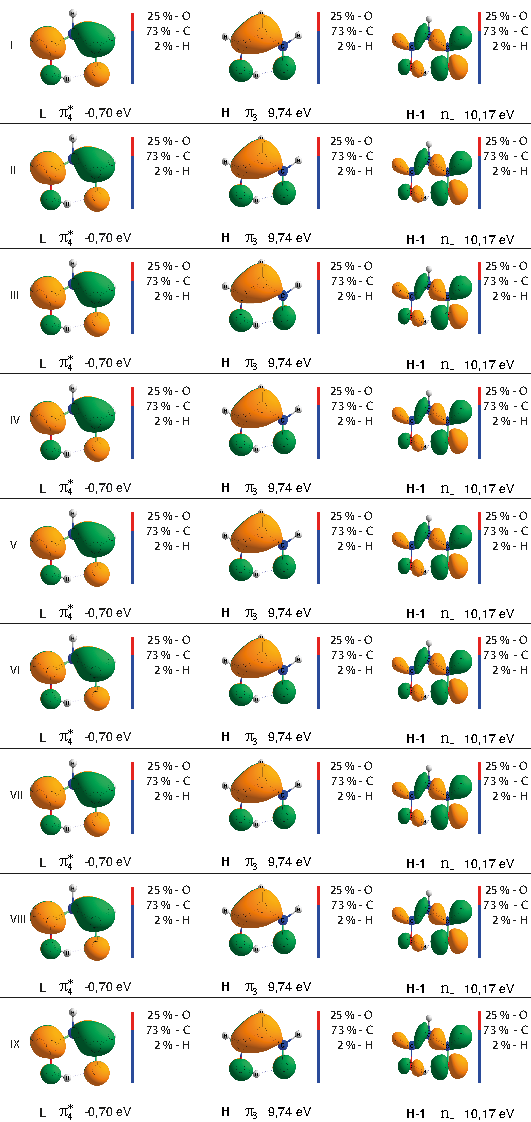
\includegraphics[width=1\linewidth]{Fig_8_top 3 orb.pdf}}
    \caption{Три верхних орбитали.}
    \label{Ris_8_orbitals}
    \end{figure}

\lipsum[14-15]

\begin{figure*}[ht]
    \center{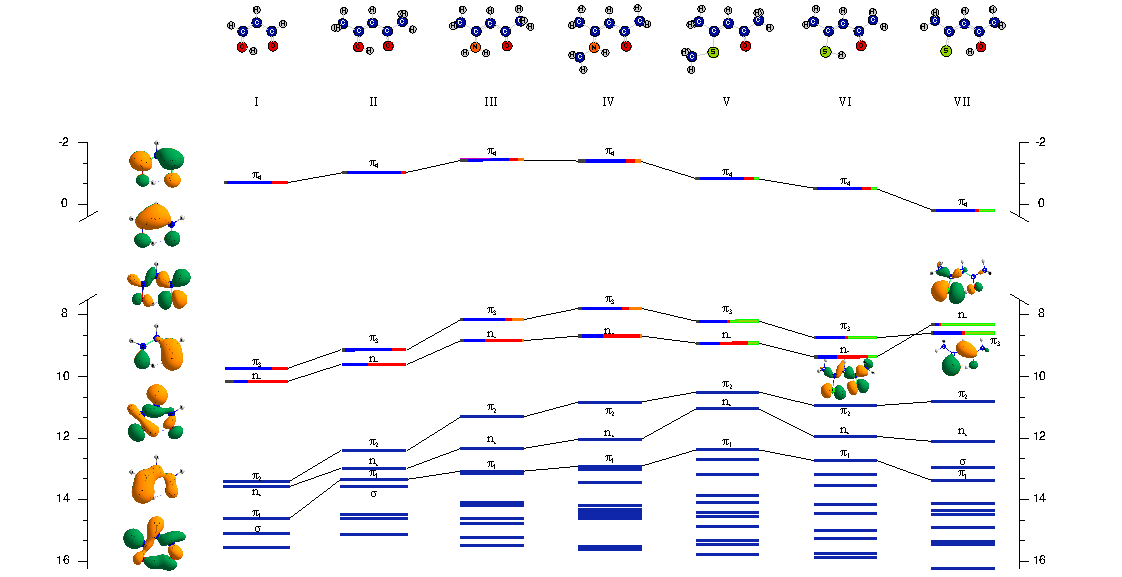
\includegraphics[width=1\linewidth]{Fig_9_diagramma.pdf}}
    \caption{Корреляционная диаграмма.}
    \label{Ris_9_diagramma_big}
    \end{figure*}

\lipsum[15-16]

\begin{figure}[ht]
    \center{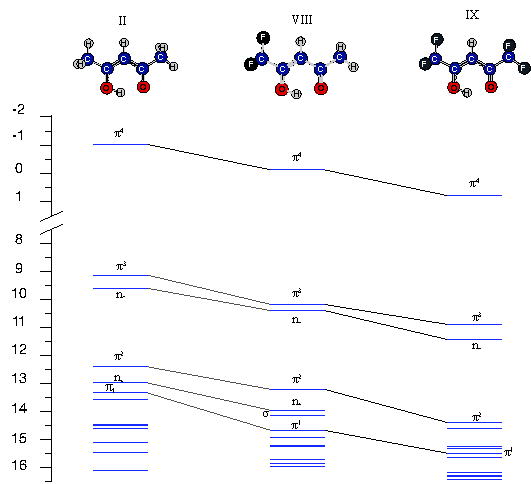
\includegraphics[width=1\linewidth]{Fig_10_small_diagramma.pdf}}
    \caption{Малая диаграмма.}
    \label{Ris_10_diagramma_small}
    \end{figure}

% Please add the following required packages to your document preamble:
% \usepackage{booktabs}
% \usepackage{multirow}

% Please add the following required packages to your document preamble:
% \usepackage{booktabs}
% \usepackage{multirow}

\begin{table}[t]
    \begin{tabular}{cclcccccc}
    \hline
                        &                       &  MO     & type          & P3+    & Exp.                      & O  & C  & H  \\ \cline{3-9}
    \multirow{8}{*}{I}  & \multirow{4}{*}{Enol} &L      &   $\pi_4$       & -0,699 &                           & 25 & 73 & 2  \\
                        &                       &H      &   $\pi_3$       & 9,74   & 9,79                      & 34 & 65 & 1  \\
                        &                       &H-1    &   n$_-$         & 10,17  & 10,24                     & 68 & 19 & 13 \\
                        &                       &H-2    &   $\pi_2$       & 13,41  & 13,23                     & 55 & 29 & 16 \\ \cline{2-9}
                        & \multirow{4}{*}{Keto} &L      &   -             & -1,02  &                           & 24 & 57 & 19 \\
                        &                       &H      &   -             & 10,25  &                           & 58 & 29 & 13 \\
                        &                       &H-1    &   -             & 10,99  &                           & 59 & 23 & 18 \\
                        &                       &H-2    &   -             & 13,73  &                           & 56 & 33 & 11 \\ \hline
    \multirow{8}{*}{II} & \multirow{4}{*}{Enol} &L      &   $\pi_4$       & -1,03  &                           & 22 & 71 & 7  \\
                        &                       &H      &   $\pi_3$       & 9,13   & \multicolumn{1}{l}{9,08}  & 30 & 67 & 3  \\
                        &                       &H-1    &   n$_-$         & 9,61   & \multicolumn{1}{l}{9,69}  & 67 & 29 & 4  \\
                        &                       &H-2    &   $\pi_2$       & 12,40  & \multicolumn{1}{l}{12,50} & 57 & 29 & 14 \\ \cline{2-9}
                        & \multirow{4}{*}{Keto} &L      &   -             & -1,246 &                           & 21 & 42 & 37 \\
                        &                       &H      &   -             & 9,711  & \multicolumn{1}{l}{9,60}  & 54 & 42 & 4  \\
                        &                       &H-1    &   -             & 10,157 & \multicolumn{1}{l}{10,16} & 59 & 35 & 7  \\
                        &                       &H-2    &   -             & 12,889 &                           & 51 & 32 & 17 \\ \hline 
    \end{tabular}
    \end{table}


    \begin{table}[t]
        \caption{Таблица I-IV}
        \begin{tabular}{@{}cccccccc@{}}
        \toprule

    &  &        &                           & III  &    &    &    \\ \midrule
    &  & P3+    & Exp.                      & O             & C  & H  & N  \\ \midrule
    &  & -1,438 &                           & 14            & 65 & 11 & 10 \\ \midrule
    &  & 8,16   & \multicolumn{1}{l}{8,24}  & 13            & 60 & 3  & 24 \\ \midrule
    &  & 8,83   & \multicolumn{1}{l}{8,98}  & 65            & 28 & 5  & 2  \\ \midrule
    &  & 11,32  & \multicolumn{1}{l}{11,21} & 31            & 30 & 10 & 29 \\ \midrule
    &  &        &                           & IV &    &    &    \\ \midrule
    &  & P3+    & Exp.                      & O             & C  & H  & N  \\ \midrule
    &  & -1,403 &                           & 14            & 65 & 11 & 10 \\ \midrule
    &  & 7,79   & \multicolumn{1}{l}{7,81}  & 13            & 57 & 6  & 24 \\ \midrule
    &  & 8,68   & \multicolumn{1}{l}{8,74}  & 65            & 28 & 5  & 2  \\ \midrule
    &  & 10,83  & \multicolumn{1}{l}{10,59} & 26            & 34 & 14 & 26 \\ \bottomrule

\end{tabular}
\end{table}


\begin{table}[t]
    \caption{Таблица V-IX}
    \begin{tabular}{@{}ccccccll@{}}
    \toprule
           &       & V – CH3Sacac  &    &    &    &  &  \\
    P3+    & Exp.  & O             & C  & H  & S  &  &  \\\midrule
    -0,83  &       & 15            & 71 & 5  & 9  &  &  \\
    8,21   & 8,54  & 6             & 40 & 4  & 50 &  &  \\
    8,91   & 9,03  & 61            & 28 & 3  & 8  &  &  \\
    10,51  & 10,57 & 17            & 45 & 9  & 29 &  &  \\\midrule
           &       & VI – HS\_Hac  &    &    &    &  &  \\
    P3+    & Exp.  & O             & C  & H  & S  &  &  \\\midrule
    -0,516 &       & 15            & 71 & 5  & 9  &  &  \\
           & 8,55  &               &    &    &    &  &  \\
    8,75   & 8,73  & 7             & 42 & 2  & 49 &  &  \\
    9,37   & 9,29  & 59            & 26 & 5  & 10 &  &  \\
    10,95  & 10,77 & 13            & 43 & 8  & 36 &  &  \\\midrule
           &       & VII – S\_OHac &    &    &    &  &  \\
    P3+    & Exp.  & O             & C  & H  & S  &  &  \\\midrule
    0,19   &       & 6             & 63 & 6  & 25 &  &  \\
    8,32   & 8,55  & 6             & 8  & 4  & 82 &  &  \\
    8,59   & 8,73  & 8             & 45 & 3  & 44 &  &  \\
           & 9,29  &               &    &    &    &  &  \\
    10,82  & 10,77 & 13            & 52 & 9  & 26 &  &  \\\midrule
           &       & VIII – Htfac  &    &    &    &  &  \\
    P3+    & Exp.  & O             & C  & H  & F  &  &  \\\midrule
    -0,122 &       & 23            & 73 & 2  & 2  &  &  \\
    10,18  & 10,01 & 33            & 65 & 1  & 1  &  &  \\
    10,41  & 10,60 & 66            & 29 & 4  & 1  &  &  \\
    13,22  & 13,31 & 52            & 31 & 16 & 1  &  &  \\\midrule
           &       & IX –Hhfac     &    &    &    &  &  \\
    P3+    & Exp.  & O             & C  & H  & F  &  &  \\\midrule
    0,81   &       & 26            & 71 & 0  & 3  &  &  \\
    10,90  & 10,85 & 34            & 64 & 1  & 1  &  &  \\
    11,44  & 11,41 & 61            & 29 & 2  & 8  &  &  \\
    14,61  & 14,20 & 32            & 34 & 8  & 26 &  &  \\\bottomrule 
    \end{tabular}
    \end{table}

\section{Summary}
\section*{Credit authorship contribution statement}
\section*{Declaration of competing interests}
\section*{Acknowledgements}
\section*{Appendix A. Supplementary data}
\begin{figure}[ht]
    \center{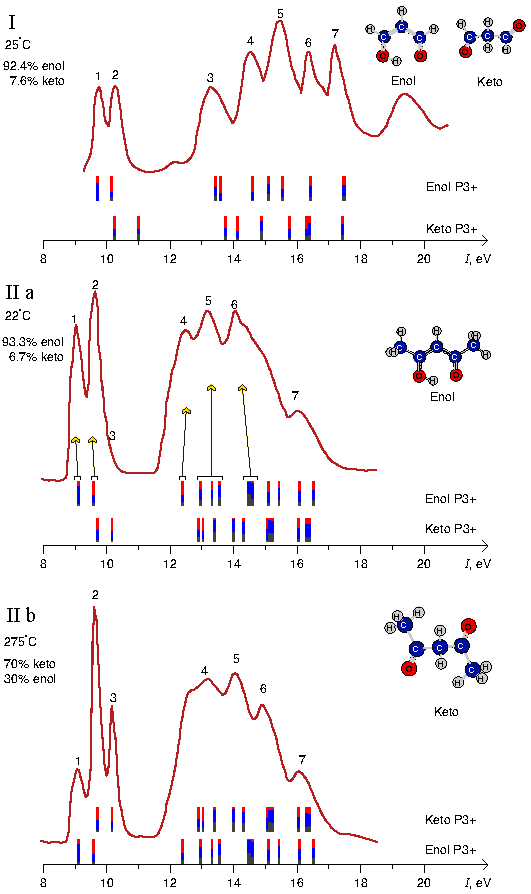
\includegraphics[width=1\linewidth]{app_1_UPS_met_1 .pdf}}
    \caption{Сравнение методов 1.}
    \label{app_1_sravnenie}
    \end{figure}

    \begin{figure}[ht]
    \center{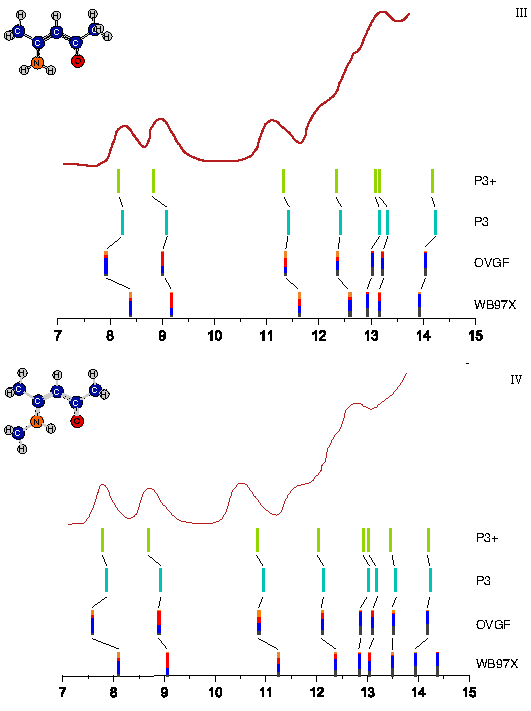
\includegraphics[width=1\linewidth]{app_2_UPS_met_2 .pdf}}
    \caption{Сравнение методов 2.}
    \label{app_2_sravnenie}
    \end{figure}

    \begin{figure}[ht]
    \center{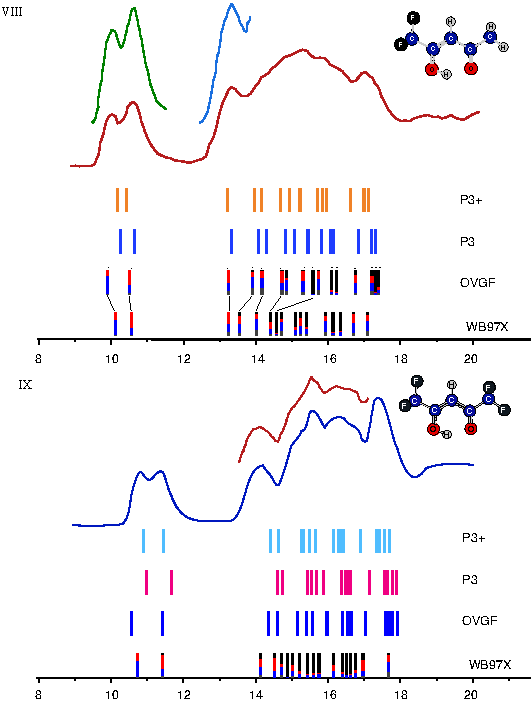
\includegraphics[width=1\linewidth]{app_3_UPS_met_3 .pdf}}
    \caption{Сравнение методов 3.}
    \label{app_3_sravnenie}
    \end{figure}

\printcredits

%% Loading bibliography style file
\bibliographystyle{model1-num-names}
%\bibliographystyle{cas-model2-names}

% Loading bibliography database
\bibliography{cas-refs}



\end{document}

